%% Patent Application: Delivery Hardware for Resonant Protein Folding Modulation
%% in Biological Contexts
%% Inventor: Jonathan Washburn
%% Contact: washburn.jonathan@gmail.com
%% Filing Date: January 2026

\documentclass[12pt,letterpaper]{article}

\usepackage[margin=1in]{geometry}
\usepackage{amsmath,amssymb,amsfonts}
\usepackage{graphicx}
\usepackage{tikz}
\usetikzlibrary{shapes,arrows,positioning,calc,patterns,decorations.pathmorphing}
\usepackage{booktabs}
\usepackage{array}
\usepackage{enumitem}
\usepackage{fancyhdr}
\usepackage{xcolor}
\usepackage{hyperref}
\usepackage{setspace}

% Patent-style formatting
\setlength{\parindent}{0.5in}
\setlength{\parskip}{0.5em}
\onehalfspacing

% Header
\pagestyle{fancy}
\fancyhf{}
\rhead{Patent Application}
\lhead{Washburn}
\rfoot{Page \thepage}

\hypersetup{
    colorlinks=true,
    linkcolor=blue,
    urlcolor=blue,
    citecolor=blue
}

% Custom colors
\definecolor{metal}{RGB}{150,150,170}
\definecolor{dielectric}{RGB}{200,220,255}
\definecolor{sample}{RGB}{255,200,200}
\definecolor{field}{RGB}{255,150,50}

\begin{document}

%% ============================================================================
%%                              TITLE PAGE
%% ============================================================================

\begin{center}
\vspace*{0.8in}

{\LARGE \textbf{PATENT APPLICATION}}

\vspace{0.4in}

{\Large \textbf{DELIVERY HARDWARE FOR RESONANT}}

{\Large \textbf{PROTEIN FOLDING MODULATION IN}}

{\Large \textbf{BIOLOGICAL CONTEXTS}}

\vspace{0.8in}

\textbf{PROVISIONAL PATENT APPLICATION}

\vspace{0.5in}

\begin{tabular}{ll}
\textbf{Inventor:} & Jonathan Washburn \\
\textbf{Email:} & washburn.jonathan@gmail.com \\
\textbf{Filing Date:} & January 17, 2026 \\
\textbf{Application Type:} & Utility Patent (Provisional) \\
\textbf{Related Applications:} & Patents 001--007 \\
\end{tabular}

\vspace{0.8in}

\textit{Hardware components for delivering resonant microwave radiation at the molecular gate frequency (10--20 GHz) to biological samples, including specialized applicators (waveguide cuvettes, microfluidic chambers, near-field antennas, resonant cavities), electromagnetic shielding, calibration phantoms, and dosimetry systems.}

\vfill

\textbf{CONFIDENTIAL --- PATENT PENDING}

\end{center}

\newpage

%% ============================================================================
%%                         TABLE OF CONTENTS
%% ============================================================================

\tableofcontents
\newpage

%% ============================================================================
%%                              ABSTRACT
%% ============================================================================

\section*{ABSTRACT OF THE DISCLOSURE}
\addcontentsline{toc}{section}{ABSTRACT OF THE DISCLOSURE}

Hardware components for delivering resonant microwave radiation at the molecular gate frequency (10--20 GHz, specifically $\sim$14.65 GHz for H$_2$O and $\sim$10.4 GHz for D$_2$O) to biological samples for protein folding modulation. The hardware comprises: (a) waveguide-coupled cuvette applicators for bench-top research; (b) microfluidic flow chambers for continuous processing and kinetic studies; (c) near-field antenna applicators for localized delivery to cells, tissues, or in-vivo applications; (d) resonant cavity applicators for high-efficiency bulk processing; (e) electromagnetic shielding enclosures to contain radiation and prevent interference; (f) calibration phantoms with defined dielectric properties for system verification; and (g) dosimetry systems for measuring and controlling delivered power. The hardware is specifically designed for the 10--20 GHz frequency range relevant to protein folding modulation, with features including optical access for fluorescence detection, temperature control integration, isotope-compatible materials, and modular construction for flexibility. Applications include laboratory research instruments, biopharmaceutical manufacturing equipment, and potential therapeutic delivery devices. All hardware maintains electromagnetic emission levels below regulatory limits while enabling efficient energy delivery to biological samples.

\vspace{1em}
\noindent\textbf{Keywords:} microwave applicator, waveguide, microfluidic, near-field antenna, resonant cavity, shielding, calibration phantom, dosimetry, protein folding, 10--20 GHz

\newpage

%% ============================================================================
%%                      BACKGROUND OF THE INVENTION
%% ============================================================================

\section{BACKGROUND OF THE INVENTION}

\subsection{Field of the Invention}

The present invention relates generally to hardware for delivering electromagnetic radiation to biological samples, and more specifically to applicators, shielding, calibration, and dosimetry systems designed for the 10--20 GHz frequency range used in resonant protein folding modulation.

\subsection{Description of Related Art}

\subsubsection{Existing Microwave Applicator Technology}

Prior art microwave applicators are designed for different frequency ranges and applications:

\begin{table}[h]
\centering
\begin{tabular}{llll}
\toprule
\textbf{Technology} & \textbf{Frequency} & \textbf{Application} & \textbf{Limitations for PFM} \\
\midrule
Domestic ovens & 2.45 GHz & Heating & Wrong frequency, no precision \\
Industrial heating & 915 MHz, 2.45 GHz & Processing & Wrong frequency \\
Diathermy & 27 MHz, 2.45 GHz & Therapy & Wrong frequency \\
Hyperthermia & 434 MHz, 915 MHz & Cancer & Wrong frequency \\
NMR/MRI & 60--900 MHz & Imaging & Wrong frequency, different purpose \\
EPR & 9--35 GHz & Spectroscopy & Designed for spin, not folding \\
\bottomrule
\end{tabular}
\caption{Existing microwave applicator technologies (PFM = protein folding modulation)}
\end{table}

\subsubsection{Limitations of Prior Art}

\begin{enumerate}[label=(\alph*)]
\item \textbf{Wrong frequency range:} Most applicators are designed for 2.45 GHz or lower; 10--20 GHz requires different waveguide sizes, materials, and design principles.

\item \textbf{No optical access:} Prior applicators are designed for heating or imaging, not combined microwave-optical experiments.

\item \textbf{Poor temperature control:} Prior applicators for biological samples often lack the precision temperature control ($\pm$0.1$^\circ$C) needed for isothermal resonant modulation.

\item \textbf{No isotope compatibility:} Prior applicators are not designed for switching between H$_2$O and D$_2$O samples with automatic frequency reconfiguration.

\item \textbf{No folding-specific design:} Prior applicators do not account for the specific requirements of protein folding experiments (denaturant compatibility, rapid mixing, kinetic measurements).
\end{enumerate}

\subsubsection{The Need for Purpose-Built Hardware}

What is needed is hardware specifically designed for:

\begin{enumerate}[label=(\arabic*)]
\item Efficient delivery of 10--20 GHz radiation to aqueous biological samples;
\item Optical access for fluorescence and other spectroscopic detection;
\item Precision temperature control with minimal heating from irradiation;
\item Compatibility with both H$_2$O and D$_2$O solvents;
\item Compatibility with folding initiation methods (mixing, temperature jump);
\item Safe operation with adequate shielding;
\item Accurate dosimetry and calibration.
\end{enumerate}

\subsection{Objects of the Invention}

It is an object of the present invention to provide hardware that:

\begin{enumerate}[label=(\arabic*)]
\item Efficiently couples 10--20 GHz radiation into biological samples;
\item Provides optical access for detection;
\item Integrates with temperature control;
\item Supports multiple sample formats (cuvette, microfluidic, tissue);
\item Includes shielding for safe operation;
\item Includes calibration and dosimetry capabilities.
\end{enumerate}

\newpage

%% ============================================================================
%%                      SUMMARY OF THE INVENTION
%% ============================================================================

\section{SUMMARY OF THE INVENTION}

\subsection{General Statement of the Invention}

The present invention provides hardware components for resonant protein folding modulation, comprising:

\begin{enumerate}[label=(\alph*)]
\item Waveguide-coupled cuvette applicators;
\item Microfluidic flow chamber applicators;
\item Near-field antenna applicators;
\item Resonant cavity applicators;
\item Electromagnetic shielding enclosures;
\item Calibration phantoms;
\item Dosimetry systems.
\end{enumerate}

\subsection{Hardware Categories}

\begin{figure}[h]
\centering
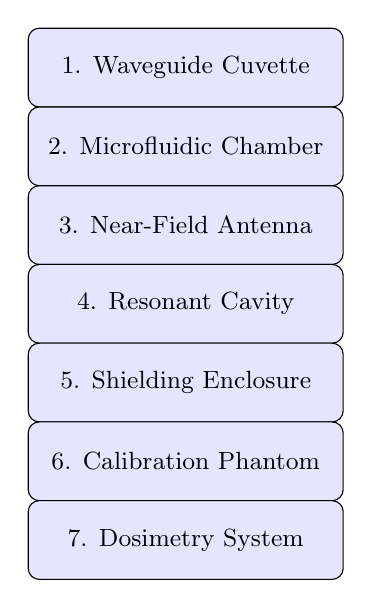
\begin{tikzpicture}[
    hw/.style={rectangle, draw, rounded corners, minimum width=4cm, minimum height=1cm, text centered, font=\small, fill=blue!10}
]
    \node[hw] at (0,5) {1. Waveguide Cuvette};
    \node[hw] at (0,4) {2. Microfluidic Chamber};
    \node[hw] at (0,3) {3. Near-Field Antenna};
    \node[hw] at (0,2) {4. Resonant Cavity};
    \node[hw] at (0,1) {5. Shielding Enclosure};
    \node[hw] at (0,0) {6. Calibration Phantom};
    \node[hw] at (0,-1) {7. Dosimetry System};
\end{tikzpicture}
\caption{Seven categories of delivery hardware}
\label{fig:categories}
\end{figure}

\subsection{Frequency Range}

All hardware is designed for operation in the 10--20 GHz range:

\begin{table}[h]
\centering
\begin{tabular}{lll}
\toprule
\textbf{Solvent} & \textbf{Target Frequency} & \textbf{Operating Range} \\
\midrule
H$_2$O & 14.65 GHz & 12--17 GHz \\
D$_2$O & 10.4 GHz & 8--13 GHz \\
\bottomrule
\end{tabular}
\caption{Target frequencies for protein folding modulation}
\end{table}

\newpage

%% ============================================================================
%%                    BRIEF DESCRIPTION OF DRAWINGS
%% ============================================================================

\section{BRIEF DESCRIPTION OF DRAWINGS}

\subsection*{Figure 1: Hardware Categories}
A list of the seven categories of delivery hardware.

\subsection*{Figure 2: Waveguide Cuvette Applicator}
Cross-sectional view showing waveguide, cuvette holder, optical ports, and thermal management.

\subsection*{Figure 3: Microfluidic Flow Chamber}
Diagram showing flow channels, microwave coupling, and detection integration.

\subsection*{Figure 4: Near-Field Antenna}
Design of antenna for localized delivery with field distribution.

\subsection*{Figure 5: Resonant Cavity}
Cylindrical cavity design with mode pattern and sample positioning.

\subsection*{Figure 6: Shielding Enclosure}
Construction details of electromagnetic shielding.

\subsection*{Figure 7: Calibration Phantom}
Phantom construction and dielectric property verification.

\subsection*{Figure 8: Dosimetry System}
Block diagram of power measurement and control system.

\newpage

%% ============================================================================
%%                      DETAILED DESCRIPTION
%% ============================================================================

\section{DETAILED DESCRIPTION OF THE PREFERRED EMBODIMENTS}

\subsection{Hardware 1: Waveguide-Coupled Cuvette Applicator}

\subsubsection{Design Overview}

The waveguide cuvette applicator couples microwave energy from a rectangular waveguide into a standard spectroscopy cuvette containing the protein sample.

\begin{figure}[h]
\centering
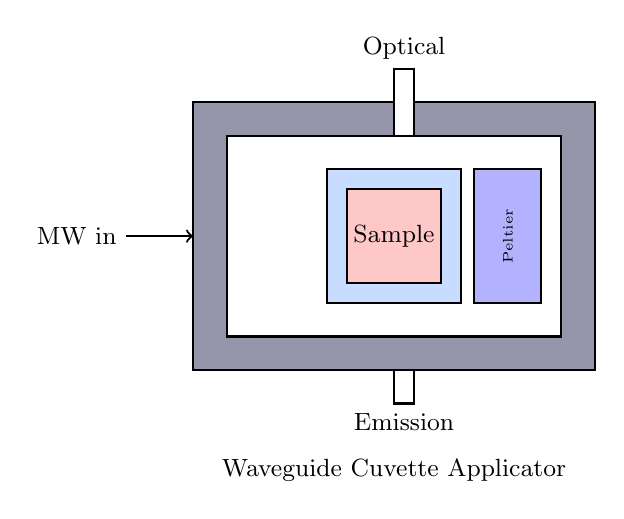
\begin{tikzpicture}[scale=0.85]
    % Waveguide
    \draw[thick, fill=metal] (0,0) rectangle (6,4);
    \draw[thick, fill=white] (0.5,0.5) rectangle (5.5,3.5);
    
    % Cuvette slot
    \draw[thick, fill=dielectric] (2,1) rectangle (4,3);
    
    % Sample
    \draw[thick, fill=sample] (2.3,1.3) rectangle (3.7,2.7);
    \node[font=\small] at (3,2) {Sample};
    
    % Optical ports
    \draw[thick, fill=white] (3,3.5) rectangle (3.3,4.5);
    \node[above, font=\small] at (3.15,4.5) {Optical};
    
    \draw[thick, fill=white] (3,0) rectangle (3.3,-0.5);
    \node[below, font=\small] at (3.15,-0.5) {Emission};
    
    % Waveguide input
    \draw[thick, ->] (-1,2) -- (0,2);
    \node[left, font=\small] at (-1,2) {MW in};
    
    % Thermal
    \draw[thick, fill=blue!30] (4.2,1) rectangle (5.2,3);
    \node[font=\tiny, rotate=90] at (4.7,2) {Peltier};
    
    % Labels
    \node[font=\small] at (3,-1.5) {Waveguide Cuvette Applicator};
    
\end{tikzpicture}
\caption{Cross-section of waveguide-coupled cuvette applicator}
\label{fig:cuvette}
\end{figure}

\subsubsection{Waveguide Specifications}

For 10--20 GHz operation, the waveguide dimensions are:

\begin{table}[h]
\centering
\begin{tabular}{lll}
\toprule
\textbf{Waveguide} & \textbf{Dimensions (a $\times$ b)} & \textbf{Frequency Range} \\
\midrule
WR-62 & 15.80 $\times$ 7.90 mm & 12.4--18.0 GHz \\
WR-75 & 19.05 $\times$ 9.53 mm & 10.0--15.0 GHz \\
WR-90 & 22.86 $\times$ 10.16 mm & 8.2--12.4 GHz \\
\bottomrule
\end{tabular}
\caption{Standard waveguide dimensions for 10--20 GHz}
\end{table}

For full coverage of 8--18 GHz, a tapered transition or dual-waveguide design is used.

\subsubsection{Cuvette Holder}

\begin{itemize}
\item Accepts standard 10 mm path-length cuvettes (quartz or UV-transparent plastic)
\item Spring-loaded retention for consistent positioning
\item Electrical isolation from waveguide walls
\item Thermal contact to Peltier element
\end{itemize}

\subsubsection{Optical Access}

\begin{itemize}
\item Top and bottom ports for fluorescence excitation/emission
\item Ports fitted with microwave-blocking mesh ($<$ 1 mm aperture)
\item Mesh transmits $>$ 90\% of 250--700 nm light
\item Optional side ports for 90$^\circ$ detection geometry
\end{itemize}

\subsubsection{Thermal Integration}

\begin{itemize}
\item Peltier element in thermal contact with cuvette holder
\item Fiber-optic temperature sensor inside cuvette
\item Heat sink with fan for Peltier hot side
\item Temperature control range: 4--50$^\circ$C
\item Stability: $\pm$0.1$^\circ$C
\end{itemize}

\subsection{Hardware 2: Microfluidic Flow Chamber}

\subsubsection{Design Overview}

The microfluidic flow chamber enables continuous processing and kinetic studies by flowing sample through a microwave irradiation zone.

\begin{figure}[h]
\centering
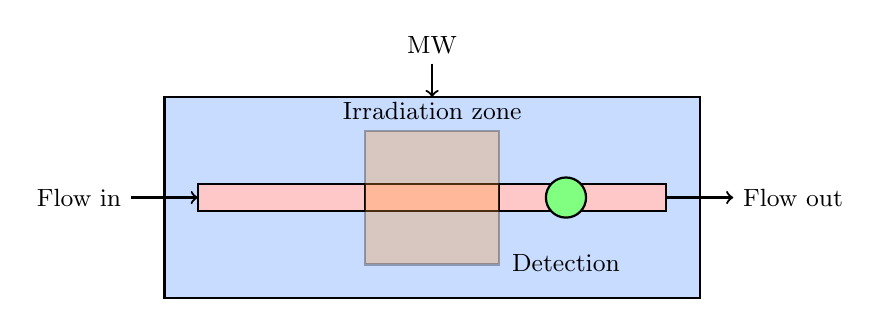
\begin{tikzpicture}[scale=0.85]
    % Chip substrate
    \draw[thick, fill=dielectric] (0,0) rectangle (8,3);
    
    % Flow channel
    \draw[thick, fill=sample] (0.5,1.3) -- (3,1.3) -- (3,1.7) -- (0.5,1.7) -- cycle;
    \draw[thick, fill=sample] (3,1.3) -- (5,1.3) -- (5,1.7) -- (3,1.7) -- cycle;
    \draw[thick, fill=sample] (5,1.3) -- (7.5,1.3) -- (7.5,1.7) -- (5,1.7) -- cycle;
    
    % Irradiation zone
    \draw[thick, fill=field, opacity=0.3] (3,0.5) rectangle (5,2.5);
    \node[font=\small] at (4,2.8) {Irradiation zone};
    
    % Microwave coupling
    \draw[thick, ->] (4,3.5) -- (4,3);
    \node[above, font=\small] at (4,3.5) {MW};
    
    % Flow arrows
    \draw[thick, ->] (-0.5,1.5) -- (0.5,1.5);
    \node[left, font=\small] at (-0.5,1.5) {Flow in};
    
    \draw[thick, ->] (7.5,1.5) -- (8.5,1.5);
    \node[right, font=\small] at (8.5,1.5) {Flow out};
    
    % Detection point
    \draw[thick, fill=green!50] (6,1.5) circle (0.3);
    \node[below, font=\small] at (6,0.8) {Detection};
    
\end{tikzpicture}
\caption{Microfluidic flow chamber for continuous processing}
\label{fig:microfluidic}
\end{figure}

\subsubsection{Channel Specifications}

\begin{table}[h]
\centering
\begin{tabular}{lll}
\toprule
\textbf{Parameter} & \textbf{Value} & \textbf{Notes} \\
\midrule
Channel width & 100--500 $\mu$m & Protein-dependent \\
Channel depth & 50--200 $\mu$m & Limits thermal gradient \\
Irradiation length & 5--20 mm & Residence time control \\
Flow rate & 1--100 $\mu$L/min & Kinetic resolution \\
Volume in zone & 0.1--2 $\mu$L & Sample efficiency \\
\bottomrule
\end{tabular}
\caption{Microfluidic channel specifications}
\end{table}

\subsubsection{Substrate Materials}

\begin{itemize}
\item \textbf{Fused quartz:} Low microwave loss, excellent optical properties
\item \textbf{Borosilicate glass:} Lower cost, adequate performance
\item \textbf{COC/COP polymers:} Low-cost, disposable, good optical
\item \textbf{PDMS:} Rapid prototyping, but higher microwave absorption
\end{itemize}

\subsubsection{Microwave Coupling}

\begin{itemize}
\item Coplanar waveguide (CPW) on chip surface
\item Stripline embedded in substrate
\item External waveguide with aperture coupling
\item Near-field antenna probe
\end{itemize}

\subsubsection{Integration Features}

\begin{itemize}
\item Mixing junction upstream for rapid initiation
\item Temperature sensors at inlet, zone, and outlet
\item Optical fiber ports for inline detection
\item Waste collection or downstream analysis
\end{itemize}

\subsection{Hardware 3: Near-Field Antenna Applicator}

\subsubsection{Design Overview}

Near-field antennas enable localized delivery of microwave energy to small volumes, including cells, tissue samples, or specific regions of larger samples.

\begin{figure}[h]
\centering
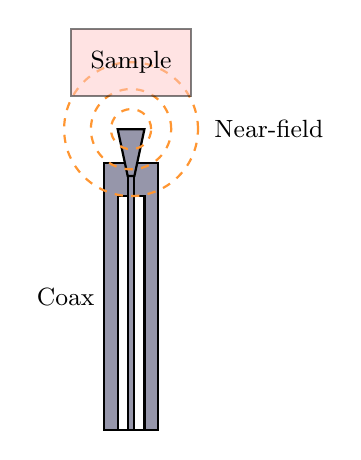
\begin{tikzpicture}[scale=0.85]
    % Coaxial feed
    \draw[thick, fill=metal] (0,0) -- (0,4) -- (0.8,4) -- (0.8,0) -- cycle;
    \draw[thick, fill=white] (0.2,0) -- (0.2,3.5) -- (0.6,3.5) -- (0.6,0) -- cycle;
    \draw[thick, fill=metal] (0.35,0) -- (0.35,3.8) -- (0.45,3.8) -- (0.45,0) -- cycle;
    
    % Antenna tip
    \draw[thick, fill=metal] (0.35,3.8) -- (0.2,4.5) -- (0.6,4.5) -- (0.45,3.8) -- cycle;
    
    % Near-field region
    \draw[thick, dashed, field] (0.4,4.5) circle (1);
    \draw[thick, dashed, field] (0.4,4.5) circle (0.6);
    \draw[thick, dashed, field] (0.4,4.5) circle (0.3);
    
    % Sample
    \draw[thick, fill=sample, opacity=0.5] (-0.5,5) rectangle (1.3,6);
    \node[font=\small] at (0.4,5.5) {Sample};
    
    % Labels
    \node[left, font=\small] at (0,2) {Coax};
    \node[right, font=\small] at (1.5,4.5) {Near-field};
    
\end{tikzpicture}
\caption{Near-field antenna for localized delivery}
\label{fig:nearfield}
\end{figure}

\subsubsection{Antenna Types}

\begin{table}[h]
\centering
\begin{tabular}{llll}
\toprule
\textbf{Type} & \textbf{Size} & \textbf{Field Pattern} & \textbf{Application} \\
\midrule
Monopole & 5--10 mm & Omnidirectional & General \\
Dipole & 10--20 mm & Bidirectional & Symmetric \\
Patch & 5$\times$5 mm & Unidirectional & Surface \\
Slot & 3$\times$10 mm & Focused & Localized \\
Aperture probe & 1--3 mm & Highly localized & Cellular \\
\bottomrule
\end{tabular}
\caption{Near-field antenna types for 15 GHz}
\end{table}

\subsubsection{Near-Field Characteristics}

For antenna dimension $a$ at frequency $f$:

\begin{equation}
\text{Near-field radius} \approx \frac{2a^2}{\lambda} = \frac{2a^2 f}{c}
\label{eq:nearfield}
\end{equation}

At 15 GHz ($\lambda = 20$ mm), a 5 mm antenna has near-field radius $\sim$2.5 mm.

\subsubsection{Applications}

\begin{enumerate}[label=(\arabic*)]
\item \textbf{Cell culture:} Irradiate specific wells in multi-well plates
\item \textbf{Tissue sections:} Localized treatment of tissue samples
\item \textbf{In-vivo (future):} Potential for localized therapeutic delivery
\item \textbf{Microscopy integration:} Combined microwave-optical imaging
\end{enumerate}

\subsection{Hardware 4: Resonant Cavity Applicator}

\subsubsection{Design Overview}

Resonant cavities provide high-efficiency coupling for bulk sample processing by matching the cavity resonance to the molecular gate frequency.

\begin{figure}[h]
\centering
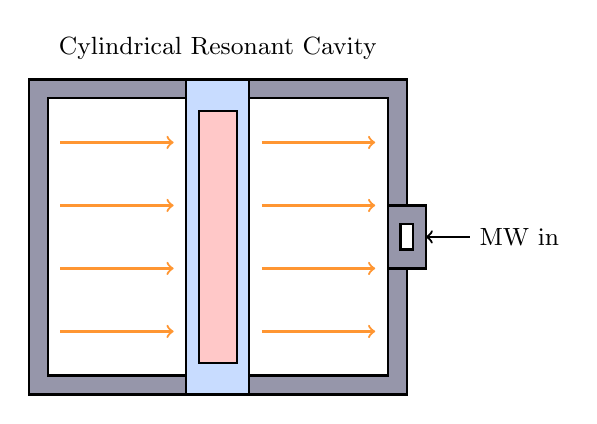
\begin{tikzpicture}[scale=0.8]
    % Cavity walls
    \draw[thick, fill=metal] (0,0) -- (0,5) -- (6,5) -- (6,0) -- cycle;
    \draw[thick, fill=white] (0.3,0.3) -- (0.3,4.7) -- (5.7,4.7) -- (5.7,0.3) -- cycle;
    
    % Sample tube
    \draw[thick, fill=dielectric] (2.5,0) -- (2.5,5) -- (3.5,5) -- (3.5,0) -- cycle;
    \draw[thick, fill=sample] (2.7,0.5) -- (2.7,4.5) -- (3.3,4.5) -- (3.3,0.5) -- cycle;
    
    % Field pattern (TE mode)
    \foreach \y in {1,2,3,4} {
        \draw[thick, field, ->] (0.5,\y) -- (2.3,\y);
        \draw[thick, field, ->] (3.7,\y) -- (5.5,\y);
    }
    
    % Coupling iris
    \draw[thick, fill=metal] (5.7,2) rectangle (6.3,3);
    \draw[thick, fill=white] (5.9,2.3) rectangle (6.1,2.7);
    
    % Input
    \draw[thick, ->] (7,2.5) -- (6.3,2.5);
    \node[right, font=\small] at (7,2.5) {MW in};
    
    % Labels
    \node[font=\small] at (3,5.5) {Cylindrical Resonant Cavity};
    
\end{tikzpicture}
\caption{Resonant cavity applicator with sample tube}
\label{fig:cavity}
\end{figure}

\subsubsection{Cavity Modes}

For a cylindrical cavity of radius $a$ and height $d$:

\begin{equation}
f_{mnp} = \frac{c}{2\pi\sqrt{\mu\epsilon}} \sqrt{\left(\frac{x'_{mn}}{a}\right)^2 + \left(\frac{p\pi}{d}\right)^2}
\label{eq:cavity}
\end{equation}

where $x'_{mn}$ is the $n$-th root of $J'_m(x) = 0$ for TE modes.

\subsubsection{Cavity Dimensions}

For TE$_{011}$ mode at 14.65 GHz:

\begin{table}[h]
\centering
\begin{tabular}{lll}
\toprule
\textbf{Parameter} & \textbf{Value} & \textbf{Notes} \\
\midrule
Radius $a$ & 12.5 mm & For $f_{011} = 14.65$ GHz \\
Height $d$ & 25 mm & $d = 2a$ for high Q \\
Sample tube ID & 5--8 mm & Standard NMR tube \\
Quality factor $Q$ & 5000--10000 & Unloaded \\
Loaded $Q$ & 500--2000 & With sample \\
\bottomrule
\end{tabular}
\caption{Resonant cavity dimensions for 14.65 GHz}
\end{table}

\subsubsection{Tuning}

\begin{itemize}
\item \textbf{Mechanical tuning:} Adjustable plunger or end plate
\item \textbf{Electronic tuning:} Varactor diode in coupling circuit
\item \textbf{Sample-dependent:} Cavity tracks sample dielectric
\end{itemize}

\subsubsection{Advantages}

\begin{enumerate}[label=(\arabic*)]
\item High efficiency: $>$90\% power into sample
\item Uniform field: Sample at field maximum
\item High Q: Low power needed for strong field
\item Stable: Temperature-compensated design possible
\end{enumerate}

\subsection{Hardware 5: Electromagnetic Shielding}

\subsubsection{Shielding Requirements}

\begin{table}[h]
\centering
\begin{tabular}{lll}
\toprule
\textbf{Standard} & \textbf{Limit} & \textbf{Notes} \\
\midrule
IEEE C95.1 & 10 mW/cm$^2$ & Occupational, 10--300 GHz \\
ICNIRP & 10 W/m$^2$ & General public, 10--300 GHz \\
FCC 47 CFR 1.1310 & 1 mW/cm$^2$ & Uncontrolled environment \\
\bottomrule
\end{tabular}
\caption{Electromagnetic exposure limits at 10--20 GHz}
\end{table}

\subsubsection{Enclosure Design}

\begin{figure}[h]
\centering
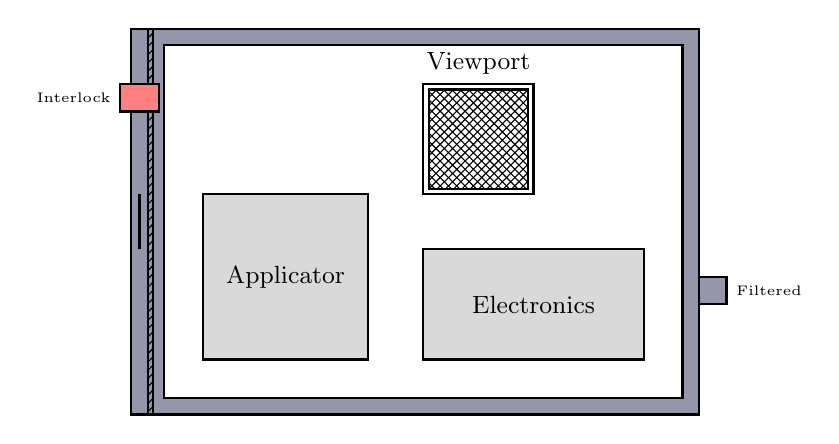
\begin{tikzpicture}[scale=0.7]
    % Outer enclosure
    \draw[thick, fill=metal] (0,0) rectangle (10,7);
    \draw[thick, fill=white] (0.3,0.3) rectangle (9.7,6.7);
    
    % Inner equipment
    \draw[thick, fill=gray!30] (1,1) rectangle (4,4);
    \node[font=\small] at (2.5,2.5) {Applicator};
    
    \draw[thick, fill=gray!30] (5,1) rectangle (9,3);
    \node[font=\small] at (7,2) {Electronics};
    
    % Door
    \draw[thick, fill=metal] (0,0) -- (0,7) -- (-0.3,7) -- (-0.3,0) -- cycle;
    \draw[thick] (-0.15,3) -- (-0.15,4);
    
    % Gasket
    \draw[thick, pattern=north east lines] (0,0) -- (0,7) -- (0.1,7) -- (0.1,0) -- cycle;
    
    % Interlock
    \draw[thick, fill=red!50] (-0.5,5.5) rectangle (0.2,6);
    \node[left, font=\tiny] at (-0.5,5.75) {Interlock};
    
    % Viewport
    \draw[thick, fill=white] (5,4) rectangle (7,6);
    \draw[thick, pattern=crosshatch] (5.1,4.1) rectangle (6.9,5.9);
    \node[above, font=\small] at (6,6) {Viewport};
    
    % Cable entry
    \draw[thick, fill=metal] (10,2) -- (10.5,2) -- (10.5,2.5) -- (10,2.5) -- cycle;
    \node[right, font=\tiny] at (10.5,2.25) {Filtered};
    
\end{tikzpicture}
\caption{Shielding enclosure with safety features}
\label{fig:shielding}
\end{figure}

\subsubsection{Shielding Effectiveness}

For aluminum enclosure at 15 GHz:

\begin{equation}
SE = 20\log_{10}\left(\frac{E_{\text{incident}}}{E_{\text{transmitted}}}\right) > 60 \text{ dB}
\label{eq:shielding}
\end{equation}

\subsubsection{Construction Details}

\begin{itemize}
\item \textbf{Material:} Aluminum (6061-T6) or steel, 1--3 mm thick
\item \textbf{Seams:} Welded or with conductive gasket (EMI gasket)
\item \textbf{Door:} Finger-stock gasket, knife-edge contact
\item \textbf{Viewports:} Conductive mesh (honeycomb, 2 mm cells)
\item \textbf{Cable entries:} Filtered feedthroughs (Pi-filter or waveguide below cutoff)
\item \textbf{Interlock:} Door switch disables power when open
\end{itemize}

\subsection{Hardware 6: Calibration Phantoms}

\subsubsection{Purpose}

Calibration phantoms are reference samples with known dielectric properties used to verify system performance and calibrate power measurements.

\subsubsection{Phantom Requirements}

\begin{table}[h]
\centering
\begin{tabular}{lll}
\toprule
\textbf{Property} & \textbf{Requirement} & \textbf{Notes} \\
\midrule
Dielectric constant $\epsilon'$ & Known $\pm$2\% & Traceable calibration \\
Loss tangent $\tan\delta$ & Known $\pm$5\% & Determines heating \\
Stability & $<$1\% change/year & Long-term reference \\
Homogeneity & $<$2\% variation & Spatial uniformity \\
Temperature coefficient & Characterized & For correction \\
\bottomrule
\end{tabular}
\caption{Calibration phantom requirements}
\end{table}

\subsubsection{Phantom Materials}

\begin{table}[h]
\centering
\begin{tabular}{llll}
\toprule
\textbf{Material} & \textbf{$\epsilon'$ at 15 GHz} & \textbf{$\tan\delta$} & \textbf{Use} \\
\midrule
Distilled water (25$^\circ$C) & $\sim$50 & $\sim$0.4 & High-loss reference \\
Saline (0.9\%) & $\sim$55 & $\sim$0.5 & Tissue-like \\
Glycerol/water & 10--50 & 0.1--0.5 & Adjustable \\
Silicone oil & 2.5 & 0.001 & Low-loss reference \\
PTFE (Teflon) & 2.1 & 0.0002 & Minimal interaction \\
Ceramic (Al$_2$O$_3$) & 9.4 & 0.0001 & Stable reference \\
\bottomrule
\end{tabular}
\caption{Calibration phantom materials at 15 GHz}
\end{table}

\subsubsection{Phantom Construction}

\begin{enumerate}[label=(\arabic*)]
\item \textbf{Liquid phantoms:} Glass or quartz container, sealed
\item \textbf{Gel phantoms:} Agar or polyacrylamide matrix with salts
\item \textbf{Solid phantoms:} Ceramic or polymer with known properties
\item \textbf{Tissue-mimicking:} Glycerol/water/NaCl mixture in gel
\end{enumerate}

\subsubsection{Verification Protocol}

\begin{enumerate}[label=(\arabic*)]
\item Measure phantom with calibrated network analyzer
\item Verify $\epsilon'$ and $\tan\delta$ against specifications
\item Use phantom to calibrate applicator power delivery
\item Verify temperature rise matches predicted heating
\item Document and store calibration data
\end{enumerate}

\subsection{Hardware 7: Dosimetry System}

\subsubsection{Dosimetry Requirements}

\begin{table}[h]
\centering
\begin{tabular}{lll}
\toprule
\textbf{Parameter} & \textbf{Requirement} & \textbf{Notes} \\
\midrule
Power range & 0.01--10 W & Covers typical experiments \\
Accuracy & $\pm$5\% & Traceable to NIST \\
Frequency range & 8--20 GHz & Covers H$_2$O and D$_2$O \\
Real-time readout & Yes & For feedback control \\
SAR calculation & Supported & Specific absorption rate \\
\bottomrule
\end{tabular}
\caption{Dosimetry system requirements}
\end{table}

\subsubsection{Measurement Methods}

\begin{enumerate}[label=(\arabic*)]
\item \textbf{Calorimetric:} Measure temperature rise in known thermal mass
\begin{equation}
P = mc_p \frac{dT}{dt}
\label{eq:calorimetric}
\end{equation}

\item \textbf{Power meter:} Directional coupler + calibrated detector
\begin{equation}
P_{\text{delivered}} = P_{\text{forward}} - P_{\text{reflected}}
\label{eq:power}
\end{equation}

\item \textbf{Field probe:} E-field sensor in sample region
\begin{equation}
\text{SAR} = \frac{\sigma |E|^2}{\rho}
\label{eq:sar}
\end{equation}
\end{enumerate}

\begin{figure}[h]
\centering
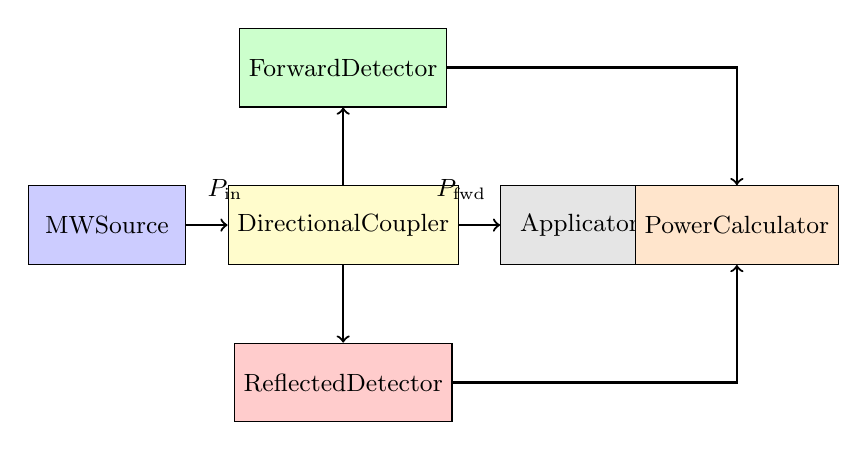
\begin{tikzpicture}[
    block/.style={rectangle, draw, minimum width=2cm, minimum height=1cm, text centered, font=\small},
    arrow/.style={->, thick}
]
    % Blocks
    \node[block, fill=blue!20] (source) at (0,2) {MW\\Source};
    \node[block, fill=yellow!20] (coupler) at (3,2) {Directional\\Coupler};
    \node[block, fill=gray!20] (app) at (6,2) {Applicator};
    \node[block, fill=green!20] (fwd) at (3,4) {Forward\\Detector};
    \node[block, fill=red!20] (ref) at (3,0) {Reflected\\Detector};
    \node[block, fill=orange!20] (calc) at (8,2) {Power\\Calculator};
    
    % Arrows
    \draw[arrow] (source) -- (coupler);
    \draw[arrow] (coupler) -- (app);
    \draw[arrow] (coupler) -- (fwd);
    \draw[arrow] (coupler) -- (ref);
    \draw[arrow] (fwd) -- (8,4) -- (calc);
    \draw[arrow] (ref) -- (8,0) -- (calc);
    
    % Labels
    \node[above, font=\small] at (1.5,2.2) {$P_{\text{in}}$};
    \node[above, font=\small] at (4.5,2.2) {$P_{\text{fwd}}$};
    
\end{tikzpicture}
\caption{Dosimetry system using directional coupler}
\label{fig:dosimetry}
\end{figure}

\subsubsection{SAR Calculation}

Specific Absorption Rate for biological samples:

\begin{equation}
\text{SAR} = \frac{P_{\text{absorbed}}}{m_{\text{sample}}} = \frac{c_p \cdot \Delta T}{\Delta t} \quad [\text{W/kg}]
\label{eq:sar_calc}
\end{equation}

\subsubsection{Dosimetry Display and Logging}

\begin{itemize}
\item Real-time display: Power (W), SAR (W/kg), Energy (J)
\item Logging: Time-stamped power profile
\item Alarms: Over-power, reflected power limit
\item Integration: Interface to control system (USB, Ethernet)
\end{itemize}

\subsection{Integrated System}

\subsubsection{Complete System Configuration}

\begin{figure}[h]
\centering
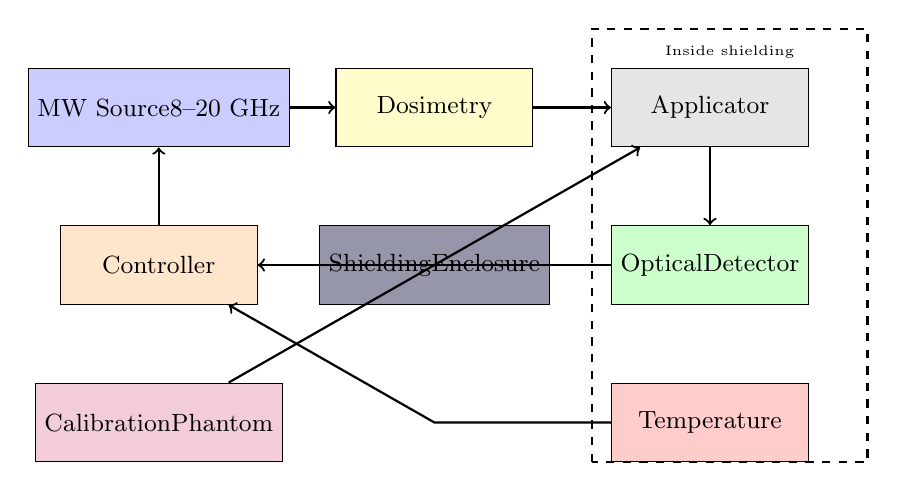
\begin{tikzpicture}[
    block/.style={rectangle, draw, minimum width=2.5cm, minimum height=1cm, text centered, font=\small},
    arrow/.style={->, thick}
]
    % Components
    \node[block, fill=blue!20] (source) at (0,4) {MW Source\\8--20 GHz};
    \node[block, fill=yellow!20] (dosimetry) at (3.5,4) {Dosimetry};
    \node[block, fill=gray!20] (applicator) at (7,4) {Applicator};
    \node[block, fill=green!20] (detector) at (7,2) {Optical\\Detector};
    \node[block, fill=red!20] (temp) at (7,0) {Temperature};
    \node[block, fill=metal] (shield) at (3.5,2) {Shielding\\Enclosure};
    \node[block, fill=orange!20] (control) at (0,2) {Controller};
    \node[block, fill=purple!20] (phantom) at (0,0) {Calibration\\Phantom};
    
    % Arrows
    \draw[arrow] (source) -- (dosimetry);
    \draw[arrow] (dosimetry) -- (applicator);
    \draw[arrow] (applicator) -- (detector);
    \draw[arrow] (detector) -- (control);
    \draw[arrow] (temp) -- (3.5,0) -- (control);
    \draw[arrow] (control) -- (source);
    \draw[arrow] (phantom) -- (applicator);
    
    % Shielding box
    \draw[thick, dashed] (5.5,-.5) rectangle (9,5);
    \node[font=\tiny] at (7.25,4.7) {Inside shielding};
    
\end{tikzpicture}
\caption{Integrated system block diagram}
\label{fig:system}
\end{figure}

\subsubsection{System Specifications}

\begin{table}[h]
\centering
\begin{tabular}{lll}
\toprule
\textbf{Parameter} & \textbf{Specification} & \textbf{Notes} \\
\midrule
Frequency range & 8--20 GHz & Covers H$_2$O and D$_2$O \\
Power range & 0.1--10 W & Adjustable \\
Temperature control & 4--50$^\circ$C, $\pm$0.1$^\circ$C & Peltier-based \\
Shielding & $>$60 dB & All frequencies \\
Optical access & 250--700 nm & Fluorescence compatible \\
Sample formats & Cuvette, microfluidic, cavity & Modular \\
Safety & Interlocked, CE marked & Regulatory compliant \\
\bottomrule
\end{tabular}
\caption{Integrated system specifications}
\end{table}

\newpage

%% ============================================================================
%%                              CLAIMS
%% ============================================================================

\section{CLAIMS}

What is claimed is:

\subsection{Waveguide Cuvette Claims}

\begin{enumerate}[label=\textbf{\arabic*.}]

\item An applicator for delivering microwave radiation to a protein sample for folding modulation, comprising:
\begin{enumerate}[label=(\alph*)]
\item a waveguide configured for operation in the frequency range of 10 to 20 GHz;
\item a cuvette holder configured to position a sample cuvette within the waveguide;
\item optical access ports configured to allow fluorescence excitation and detection while blocking microwave leakage; and
\item a thermal management element in thermal contact with the cuvette holder.
\end{enumerate}

\item The applicator of claim 1, wherein the waveguide is selected from WR-62, WR-75, and WR-90.

\item The applicator of claim 1, wherein the optical access ports comprise conductive mesh with aperture size less than 2 mm.

\item The applicator of claim 1, wherein the thermal management element comprises a Peltier thermoelectric module capable of maintaining temperature to within $\pm$0.1$^\circ$C.

\end{enumerate}

\subsection{Microfluidic Claims}

\begin{enumerate}[label=\textbf{\arabic*.}]
\setcounter{enumi}{4}

\item A microfluidic flow chamber for continuous protein folding modulation, comprising:
\begin{enumerate}[label=(\alph*)]
\item a substrate of microwave-transparent material;
\item a flow channel formed in the substrate;
\item an irradiation zone where microwave radiation is coupled into the flow channel;
\item inlet and outlet ports for sample flow; and
\item detection ports for optical monitoring of the sample.
\end{enumerate}

\item The flow chamber of claim 5, wherein the substrate is selected from fused quartz, borosilicate glass, and cyclic olefin polymer.

\item The flow chamber of claim 5, wherein the flow channel has a width of 100 to 500 micrometers and a depth of 50 to 200 micrometers.

\item The flow chamber of claim 5, further comprising a mixing junction upstream of the irradiation zone for initiating protein folding.

\end{enumerate}

\subsection{Near-Field Antenna Claims}

\begin{enumerate}[label=\textbf{\arabic*.}]
\setcounter{enumi}{8}

\item A near-field antenna applicator for localized delivery of microwave radiation, comprising:
\begin{enumerate}[label=(\alph*)]
\item an antenna element configured for operation at 10 to 20 GHz;
\item a coaxial or waveguide feed;
\item a positioning mechanism for placing the antenna in proximity to a sample; and
\item wherein the antenna delivers microwave energy to a localized region having a dimension of 1 to 10 mm.
\end{enumerate}

\item The antenna of claim 9, wherein the antenna element is selected from monopole, dipole, patch, slot, and aperture probe.

\item The antenna of claim 9, configured for integration with a microscope for combined microwave-optical experiments.

\end{enumerate}

\subsection{Resonant Cavity Claims}

\begin{enumerate}[label=\textbf{\arabic*.}]
\setcounter{enumi}{11}

\item A resonant cavity applicator for high-efficiency protein folding modulation, comprising:
\begin{enumerate}[label=(\alph*)]
\item a conductive cavity having a resonant frequency in the range of 10 to 20 GHz;
\item a sample tube holder positioning a sample at a field maximum within the cavity;
\item a coupling iris or probe for coupling microwave energy into the cavity; and
\item a tuning mechanism for adjusting the resonant frequency.
\end{enumerate}

\item The cavity of claim 12, wherein the cavity is cylindrical and configured for TE$_{011}$ mode operation.

\item The cavity of claim 12, wherein the unloaded quality factor Q is greater than 5000.

\item The cavity of claim 12, wherein the resonant frequency is approximately 14.65 GHz for H$_2$O samples or 10.4 GHz for D$_2$O samples.

\end{enumerate}

\subsection{Shielding Claims}

\begin{enumerate}[label=\textbf{\arabic*.}]
\setcounter{enumi}{15}

\item An electromagnetic shielding enclosure for protein folding modulation apparatus, comprising:
\begin{enumerate}[label=(\alph*)]
\item a conductive enclosure providing shielding effectiveness greater than 60 dB at frequencies from 10 to 20 GHz;
\item a door with conductive gasket for access;
\item a door interlock that disables microwave power when the door is open;
\item filtered feedthroughs for electrical connections; and
\item a shielded viewport for visual observation.
\end{enumerate}

\item The enclosure of claim 16, wherein the conductive enclosure is constructed of aluminum or steel with thickness of 1 to 3 mm.

\item The enclosure of claim 16, wherein the shielded viewport comprises conductive mesh or honeycomb with cell size less than 3 mm.

\end{enumerate}

\subsection{Calibration Phantom Claims}

\begin{enumerate}[label=\textbf{\arabic*.}]
\setcounter{enumi}{18}

\item A calibration phantom for verifying performance of a protein folding modulation apparatus, comprising:
\begin{enumerate}[label=(\alph*)]
\item a container of known dimensions;
\item a material having known dielectric properties at frequencies from 10 to 20 GHz; and
\item wherein the dielectric constant and loss tangent are characterized to within $\pm$5\%.
\end{enumerate}

\item The phantom of claim 19, wherein the material is selected from distilled water, saline solution, glycerol-water mixture, and tissue-mimicking gel.

\item The phantom of claim 19, further comprising a temperature sensor for correcting dielectric properties for temperature.

\end{enumerate}

\subsection{Dosimetry Claims}

\begin{enumerate}[label=\textbf{\arabic*.}]
\setcounter{enumi}{21}

\item A dosimetry system for measuring power delivered to a sample during protein folding modulation, comprising:
\begin{enumerate}[label=(\alph*)]
\item a directional coupler in the microwave path;
\item forward and reflected power detectors connected to the coupler;
\item a processor configured to compute delivered power as the difference between forward and reflected power; and
\item a display configured to show delivered power in real time.
\end{enumerate}

\item The dosimetry system of claim 22, further configured to compute and display specific absorption rate (SAR) based on sample mass.

\item The dosimetry system of claim 22, further comprising an alarm for over-power conditions.

\item The dosimetry system of claim 22, further comprising a data logger for recording power profiles.

\end{enumerate}

\newpage

%% ============================================================================
%%                         ABSTRACT
%% ============================================================================

\section*{ABSTRACT}
\addcontentsline{toc}{section}{ABSTRACT}

Hardware components for delivering resonant microwave radiation at the molecular gate frequency (10--20 GHz) to biological samples for protein folding modulation. The hardware comprises: (1) waveguide-coupled cuvette applicators with WR-62/75/90 waveguides, optical access ports with conductive mesh, and Peltier thermal management; (2) microfluidic flow chambers with quartz or polymer substrates, 100--500 $\mu$m channels, and integrated mixing junctions; (3) near-field antenna applicators (monopole, dipole, patch, slot, aperture probe) for localized delivery to 1--10 mm regions; (4) resonant cavity applicators with TE$_{011}$ mode, Q $>$ 5000, and tunable resonance at 14.65 GHz (H$_2$O) or 10.4 GHz (D$_2$O); (5) electromagnetic shielding enclosures providing $>$60 dB attenuation with door interlocks, filtered feedthroughs, and shielded viewports; (6) calibration phantoms with characterized dielectric properties (water, saline, glycerol-water, tissue-mimicking gel) for system verification; and (7) dosimetry systems using directional couplers for real-time power measurement, SAR calculation, and logging. All hardware is designed for the 10--20 GHz frequency range specific to protein folding modulation, with features including optical access for fluorescence detection, precision temperature control, isotope compatibility, and modular construction. Applications include laboratory research instruments, biopharmaceutical manufacturing equipment, and potential therapeutic delivery devices.

\vspace{1in}

\begin{center}
\textbf{--- END OF SPECIFICATION ---}
\end{center}

\newpage

%% ============================================================================
%%                         INVENTOR DECLARATION
%% ============================================================================

\section*{INVENTOR DECLARATION}
\addcontentsline{toc}{section}{INVENTOR DECLARATION}

I, Jonathan Washburn, declare that:

\begin{enumerate}[label=(\arabic*)]
\item I am the original and sole inventor of the delivery hardware described and claimed in this application.

\item I have reviewed the above specification and claims and believe them to be accurate and complete.

\item I believe the claimed invention to be novel, useful, and non-obvious over the prior art.

\item I authorize the filing of this provisional patent application to establish a priority date.
\end{enumerate}

\vspace{1in}

\noindent\textbf{Inventor Signature:} \hrulefill

\vspace{0.5in}

\noindent\textbf{Name:} Jonathan Washburn

\noindent\textbf{Email:} washburn.jonathan@gmail.com

\noindent\textbf{Date:} \hrulefill

\vspace{1in}

\begin{center}
\textit{This document is intended for provisional patent application filing purposes.\\
All information contained herein is confidential and proprietary.}
\end{center}

\end{document}
